\documentclass[11pt,a4paper,fleqn]{article} 
%%%%% general %%%%%
\usepackage[T1]{fontenc} 
\usepackage{geometry}
\geometry{a4paper, top=20mm, left=20mm, right=20mm, bottom=20mm,headsep=10mm, footskip=12mm}
\usepackage[singlespacing]{setspace} %Zeilenabstand
\usepackage{xspace} %Befehle fuer Bezeichner, damit danach Leerzeichen
%%%%% lists %%%%%%

\usepackage[alwaysadjust,flushleft]{paralist}
\usepackage{enumerate}
%%%%% graphics and tables %%%%%
%\usepackage{graphicx}
\usepackage{subfigure}
\usepackage{booktabs}
\usepackage{multirow}

%\usepackage{longtable}
\usepackage{rotating}
%\usepackage{placeins}
\usepackage{flafter} %no floating object appears in the text above the position where it is defined
%\usepackage[font=small,labelfont=bf]{caption} 
\newcommand{\ra}[1]{\renewcommand{\arraystretch}{#1}}
\usepackage{tikz}
\usepackage{pgfplots}

%%%%% Mark changes %%%%%
%\usepackage{soul}
%\setstcolor{red}
%\usepackage{cancel}
\usepackage[final]{changes}

%%%%% bibliography %%%%%
\usepackage{natbib}
\bibliographystyle{abbrvnat}
\bibpunct[, ]{(}{)}{,}{a}{}{,}%
\def\bibfont{\small}%
\def\bibsep{\smallskipamount}%
\def\bibhang{24pt}%
\def\newblock{\ }%
\def\BIBand{and}%
%%%%% math and algorithms %%%%%
\usepackage{amsmath}
\usepackage{amssymb}
%\usepackage{algorithm}
\usepackage{array}
%\newcolumntype{H}{>{\setbox0=\hbox\bgroup}c<{\egroup}@{}}
\usepackage{algorithmic}
\usepackage{fixltx2e} % text super and subscripts
%%%%% color %%%%%%
\PassOptionsToPackage{usenames,dvipsnames}{color}
%\usepackage[usenames,dvipsnames]{color}
%%%%% hyperref %%%%%%
%\usepackage{url}
%\usepackage{preview}
%\usepackage{breakurl} \% break long urls
%\usepackage[colorlinks,linkcolor=Goldenrod,citecolor=Brown]{hyperref}
\usepackage{hyperref}
% \hypersetup{
%     bookmarks=true,
%     unicode=false,
%     pdftoolbar=true,
%     pdfmenubar=true,
%     pdffitwindow=false,
%     pdfstartview={FitH},
%     pdftitle={My title},
%     pdfauthor={Author},
%     pdfsubject={Subject},
%     pdfcreator={Creator},
%     pdfproducer={Producer},
%     pdfkeywords={keyword1} {key2} {key3},
%     pdfnewwindow=true,
%     colorlinks=true,
%     linkcolor=black,
%     citecolor=black,
%     filecolor=black,
%     urlcolor=black
% }


\pgfplotsset{compat=1.12}
\allowdisplaybreaks[4]
%%%%% Math Operators %%%%%
\DeclareMathOperator*{\argmin}{arg\,min}
\DeclareMathOperator*{\argmax}{arg\,max}

\usepackage{atbegshi}% http://ctan.org/pkg/atbegshi
\AtBeginDocument{\AtBeginShipoutNext{\AtBeginShipoutDiscard}}


\begin{document}

\onehalfspacing
\title{Optimizing Air Cargo Handling at an International Airline Hub for AbOvo \\} 
\author{Ilkim Canoler\thanks{\{ilkim.canoler@rwth-aachen.de, karthikeyan.ramasubbu@rwth-aachen.de, luckshan.sivakumar@rwth-aachen.de, nikhil.kulkarni@rwth-aachen.de, shekhar.dure@rwth.aachen.de\},M.Sc. Data Analytics and Decision Science, RWTH Aachen University, Germany}  \and Karthikeyan Ramasubbu\footnotemark[1] \and Luckshan Sivakumar\footnotemark[1] \and Nikhil Kulkarni \footnotemark[1] \and Shekhar Dure\footnotemark[1]} 
$\newline$
$\newline$
\date{8th July 2019}
\maketitle
\thispagestyle{empty}


$\newline$
\begin{abstract}
	In this study, we solve an operational planning problem in the air cargo industry. In an international airline hub, all shipments which arrive at the airport and have to go to another destination need to go through two processes, namely, breaking down of the unit load devices (ULDs) that arrived in and building up of ULD for their destination flight. The final goal is that all shipments have to catch their connection flight on time. Due to the complexity of the overall problem, current practices at airlines are to split up the problem into two smaller and thus simpler problems. The goal of this paper is to solve the full planning problem using a single model. Working with our industrial partner AbOvo, we solved the problem of scheduling the break down and build up process according to the departure timings of the destination flights to ensure that all shipments reaches the flight. We formalize its requirements and the objectives. Furthermore, we develop and evaluate two different solution approaches. We solve the full planning problem by using integer linear programming.
	
$\newline$
We explore two solutions to this problem. One is the main model and the other solution is named as alternative model. The BD zone model for both the solution approaches is the same. The dierence between these two approaches is only regarding the BU zone assignment process and hence we describe only the alternative BU zone model.


\textbf{Keywords:} \textit{Time Discretization,}.
	
\end{abstract}

\clearpage
\pagenumbering{arabic} 

\newpage

\tableofcontents

\newpage

\section{Introduction}
\label{sec:introduction}

$\newline$
An international airline hub needs to plan the air cargo movement so that all shipments catch their connecting flights or road connections. Air cargo shipments are transported in so-called unit load devices (ULDs). It allows a large quantity of cargo to be bundled into a single unit like a pallet or a container. A ULD may contain many shipments which need to go to different final destinations. Hence, at the first step of the whole process as seen in Figure 1 below, the incoming ULDs are broken down on arrival. Here in the breakdown zone (BD), ULDs have to be unpacked and seperated. The seperate shipments are then transported to the warehouse and stored there. These shipments are then moved to the packing area which is called buildup zone (BU). Finally, the outbound ULDs are constructed from these shipments, and they are taken to the outbound flight for loading. Each zone has different attributes such as capacitiy for BD zone, the number of workstations for BU zone, transportation times between zones and the warehouse and handling times for process in each zone. Shipments have different attributes namely shipment id, destination flight number, date of arrival and departure, type of shipment and weight. Using all the attributes , we formulate the problem as an Integer linear program by writing constraints and the parameters which are stated in detail in the problem description section. The goal of the optimization process is to build up all ULDs such that there is sifficient time available for them to catch their flight connections.

%\noindent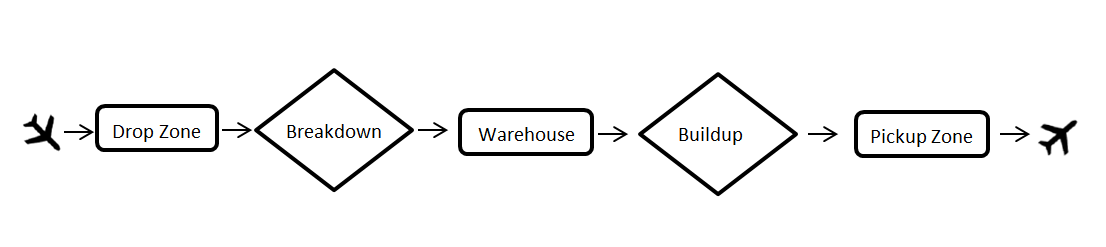
\includegraphics[width=18cm]{1_process.png}\qquad

\begin{figure}[hbt!]
	\centering
	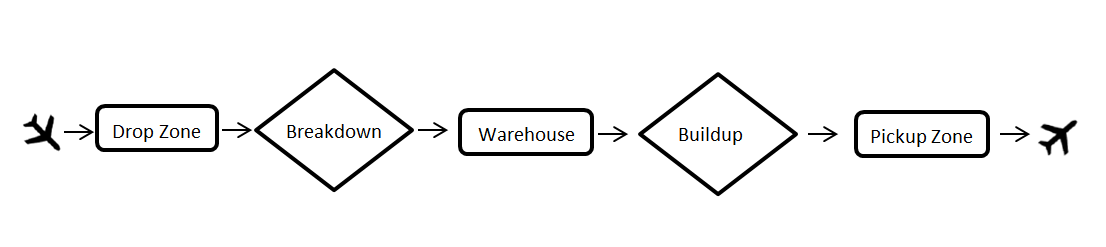
\includegraphics[width=170mm,scale=1.5]{1_process.PNG}
	\caption{The Process That Takes Place at a Hub}
	\label{fig:The Process That Takes Place at a Hub}
\end{figure}

\section{Problem Description}
\label{sec:problemdescription}

$\newline$
In the given problem, shipments arrive in the form of an ULD at four types of Drop Zones (DZ) in the airport. ULDs are unloaded from an aircraft by the ground handling agent and placed in one of the drop zones. The decision to assign the DZ is not a part of our planning problem in this paper as it has already been given in the data associated with each shipment. From the drop zone, each ULD has to be transported to the breakdown zone to be broken down into shipments. The decision of allocating an ULD to a BD zone has to be taken at this point.

%The sample distances between some of the drop zones and some of the BD zones are given below in the Figure 2.

%\newpage

%\noindent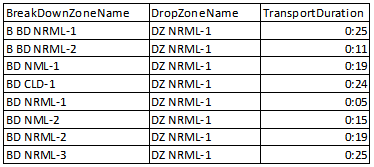
\includegraphics[width=12cm]{distances_drop_bdzone.png}\qquad

%\begin{figure}[hbt!]
%	\centering
%	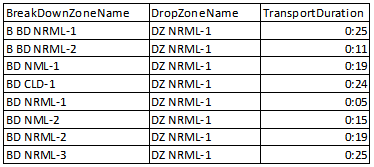
\includegraphics[width=100mm,scale=1.5]{distances_drop_bdzone.png}
%	\caption{Sample Distances Between Drop Zone and Break Down Zone}
%	\label{fig:Sample Distances Between Drop Zone and Break Down Zone}
%\end{figure}

$\newline$
In BD zone, ULDs are seperated into shipments. There are 12 different BD zones in the hub that are located at different places of the airport. Attributes related to BD zones are: 

\begin{itemize}
	\item Type of shipment a BD zone handles. For examle  : some of the BD zones handle only ULDs containing animals, some of them handle only cooled products and others handle regular ULDs.
	\item Capacity of the BD zone.
	\item Transportation times from DZ and to Warehouse.
	\item Handling time per ULD.
\end{itemize}

%\begin{figure}[hbt!]
%	\centering
%	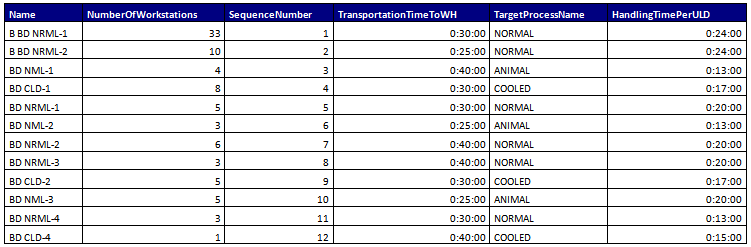
\includegraphics[width=150mm,scale=1.0]{BDZones.png}
%	\caption{Break Down Zone Attributes}
%	\label{fig:Break Down Zone Attributes}
%\end{figure}

%\noindent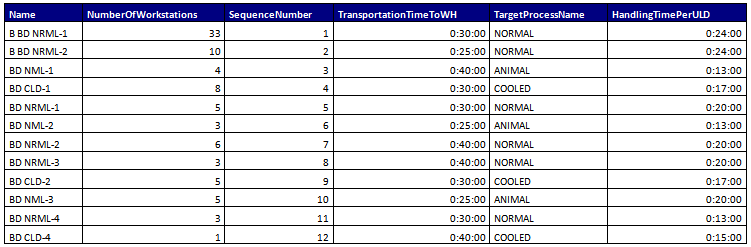
\includegraphics[width=30cm]{BDZones.png}\qquad

The inbound ULDs are classified into product categories of, 'Cooled', 'normal' and 'animals'. When the shipments are unpacked, depending on the scheduled departure time of the connection flight it is booked for, it is either stored temporarily in the warehouse or directly sent to the build up process. The warehouse (WH) is fully automated and with the assumption, that there are never capacity constraints in the WH. As soon as enough stock is available in the storage WH to build up one ULD for a specific aircraft, these can be requested to be provided to the BU zone.

$\newline$
In a next step, shipments are built up into ULDs depending on their connecting flight. This is done in a build up zone (BU zone). A departing aircraft type has a link to a specific BU zone. So with the provided information on which aircraft the shipment should go on, the BU zone is known. There are 8 different BU zones and each BU zone has different number of workstations in it. At each work station only one ULD can be built up at any given time. The shipments are provided from the storage WH to the chosen work station. From each BU zone, there are different transportation times for ULDs to each flight. In addition to this, there are different pre-processing times for each flight which is also given in the data. Maximum capacity by weight that each built up ULD can have is given as 400 kg.

Some other requirements are that if the building up of two ULDs for the same aircraft are planned at one work station, it is not allowed to build up a ULD for a different aircraft in between, even if there is some idle time. The reason is that after building up one ULD there might be some shipments with the same destination left. It should be avoided to move those around, so they would stay at the work station for the build up of the next ULD for the same aircraft. Listen below are attributes associated with BU zone

\begin{itemize}
	\item Handling times to buildup a ULD 
	
	%\begin{figure}[hbt!]
	%	\centering
	%	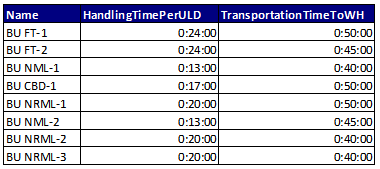
\includegraphics[width=100mm,scale=1.5]{buzone_data1.png}
	%	\caption{Handling Times and Transportation Times from Warehouse to BU Zones}
	%	\label{fig:Handling Times and Transportation Times from Warehouse to BU Zones}
	%\end{figure}

\end{itemize}

	%%\noindent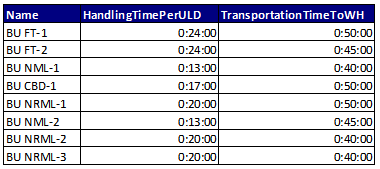
\includegraphics[width=14cm]{buzone_data1.png}\qquad
\begin{itemize}
	\item Transport times from the WH
\end{itemize}


\begin{itemize}

	\item Number of workstations
	
%	\begin{figure}[hbt!]
	%	\centering
	%	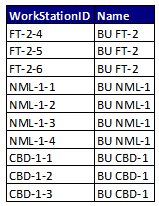
\includegraphics[width=40mm,scale=1.0]{sample_ws_bu.png}
	%	\caption{Workstations in BU Zones}
	%	\label{fig:Workstations in BU Zones}
%	\end{figure}
	%%\noindent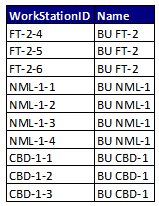
\includegraphics[width=8cm]{sample_ws_bu.png}\qquad

\end{itemize}

\begin{itemize}

	\item Flights list associated with each BU zones and the transportation time between the flight and the BU zone.
	
	%\begin{figure}[hbt!]
	%	\centering
	%	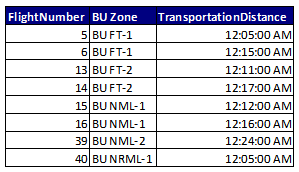
\includegraphics[width=90mm,scale=1.5]{sample_bu_flight.png}
	%	\caption{Sample Flights Related to BU Zones and Transpotation Times}
	%	\label{fig:Sample Flights Related to BU Zones and Transpotation Times}
%	\end{figure}
	%%\noindent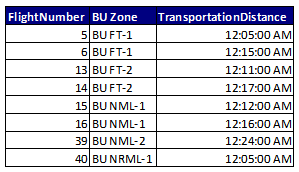
\includegraphics[width=10cm]{sample_bu_flight.png}\qquad

\end{itemize}

\begin{itemize}

	\item Pre-processing buffer times for the flights.
	
	%\begin{figure}[hbt!]
	%	\centering
	%	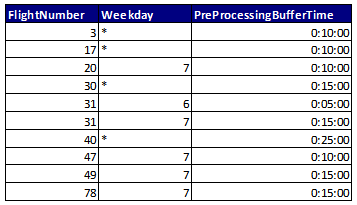
\includegraphics[width=90mm,scale=1.5]{preprocess_time.png}
	%	\caption{Pre-Processing Times of the Flights}
	%	\label{fig:Pre-Processing Times of the Flights}
%	\end{figure}
	%%\noindent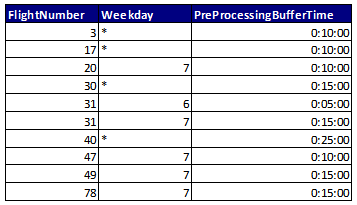
\includegraphics[width=10cm]{preprocess_time.png}\qquad
	
\end{itemize}

The goal is to build up all ULDs before the given buffer time so that all can catch the connections.

%\newpage


\section{Mathematical Model for the Problem}
\label{sec:mathmodel}

Our mathematical model for this problem is a combination of two puzzles namely, the Break Down Zone and the Build Up Zone assignments. The overall view of the general process can be seen in Figure 2 below.

$\newline$ 

\begin{figure}[hbt!]
	\centering
	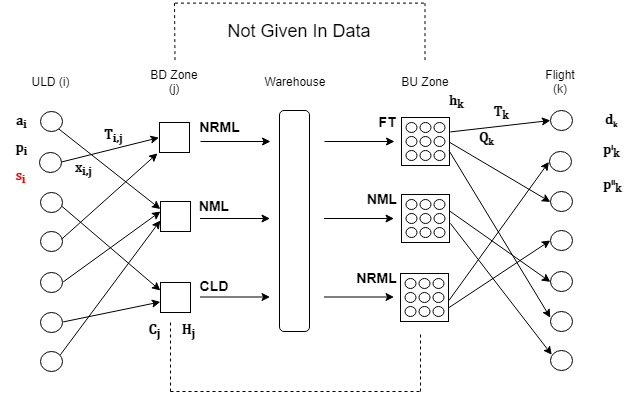
\includegraphics[width=170mm,scale=1.5]{Aircargo_overall.png}
	\caption{Overall View for The Aircargo Process}
	\label{fig:Overall View for The Aircargo Process}
\end{figure}

\subsection{Break Down Process}
\label{sec:ParamBDZone}

Each ULD is a part of the ULD set I and each BD zone is a part of the BD zones set J. Time is discretized into minutes in set T.

\begin{equation*} ${\color{black} ULD i}$ {}  \in {}  ${\color{black}I}$ {} = {} ${\color{black}\{1,2,3,...,N\}}$  \end{equation*} 
\begin{equation*} ${\color{black} BD zone j}$ {}  \in {}  ${\color{black}J}$ {} = {} ${\color{black}\{1,2,3,...,M\}}$ \end{equation*} 
\begin{equation*} ${\color{black} Time horizon t}$ {}  \in {}  ${\color{black}T}$ {} = {} ${\color{black}\{1,2,3,...,T\}}$ \end{equation*}
\begin{equation*} ${\color{black} Shipments l in ULD i}$ {}  \in {}  ${\color{black}Li}$ {} = {} ${\color{black}\{1,2,3....,L\}}$ \end{equation*} %newly_added_by_ilkim% 


${\color{black}a_{i}}$ : Arrival time of ULD ${\color{black}i}$ in drop zone 

${\color{black}d_{i}}$ : Earliest Departure time of a shipment in ULD ${\color{black}i}$ 

%$\textcolor{black}{s_{i}}$ : Idle time spent by ULD ${\color{black}i}$ in drop zone

%$\textcolor{black}{p_{i}}$ : Priority of ULD ${\color{black}i}$

${\color{black}c_{j}}$ : Capacity of BD zone ${\color{black}j}$

$\textcolor{black}{h_{j}}$ : Handling time in BD zone ${\color{black}j}$

$\textcolor{black}{T_{ij}}$ : Time taken to transport an ULD ${\color{black}i}$ to BD zone ${\color{black}j}$

$\textcolor{black}{T_{j}}$ : Time taken to transport shipments from ${\color{black}i}$ to BD zone ${\color{black}j}$ to Warehouse


\subsubsection{Decision Variables for Break Down Process}
\label{sec:DVBDZone}

In the Break Down zone, the decision needs to be taken which ULDs should be assigned to which BD zone at which time. For this reason, the decision variable has to be binary. The decision variable takes value 1 if the ULD i is assigned to BD zone j at time t and value 0 if the ULD i is not assigned to BD zone j at time t. 

$\newline$

$\textcolor{black}{x_{ij}^{t}\in\{0,1\}, \forall {i \in I, j \in J, t \in T}}$ : if a ULD i is assigned to BD zone j at time t or not.


\subsubsection{Constraints for Break Down Process}
\label{sec:constraintsBDZone}

The first constraint (1) ensures that the ULD is assigned at a feasible time, the second constraint (2) ensures that all ULDs have to be assigned to exactly one BD zone.

$\newline$
The time at which Break down of  ULD i starts, $t_{i,start} = \sum_{j \in J}\sum_{t=a_{i}}^{d_{i}} t \cdot x_{ij}^t $
$\newline$
$\newline$
Each ULD takes i  $T_{ij}$ time to travel to its assigned BD zone j, therefore the following constraint ensures that the start time of ULD i is greater than the sum of its arrival time and transportation time :
$\newline$
\begin{align}
\sum_{j \in J}\sum_{t=a_{i}}^{d_{i}} (t- T_{ij}) \cdot x_{ij}^t \ge a_{i} ,  \qquad \forall i \in I
\end{align}

Each ULD i must be assigned to a BD zone j before the earliest departure time of the shipment it contains. We will further tighten this time limit in other constraints that follow. The following constraint ensures that each ULD is assigned : 

\begin{align}
\sum_{j \in J}\sum_{t=a_{i}}^{d_{i}} x_{ij}^{t} = 1 \qquad \forall i \in I
\end{align}

For the special case given in this problem, where we have multiple drop zones, the each ULD has to be assigned to multiple BD zones associated with it. In the constraints (3) and (4), we assign such multiple drop zone ULDs to their respective BD zones i.e animal BD zone and normal BD zone.
\begin{align}
\sum_{j \in J_{NML}}\sum_{t=a_{i}}^{d_{i}} x_{ij}^{t} = 1 \qquad \forall i \in I
\end{align}

\begin{align}
\sum_{j \in J_{NRML}}\sum_{t=a_{i}}^{d_{i}} x_{ij}^{t} = 1 \qquad \forall i \in I
\end{align}

In the fifth consraint (5), we consider the case that for multiple drop zone ULDs, animal BD zone has to be assigned before the regular shipment BD zone.

$J_{NML} \bigcup J_{NRML} = J$

\begin{align}
\sum_{j\in J_{NML}}\sum_{t=a_{i}}^{d_{i}} (t + h_{j}) \cdot x_{ij}^t  \le \sum_{j\in J_{NRML}}\sum_{t=a_{i}}^{d_{i}} (t) \cdot x_{ij}^t
\end{align}


$\newline$
The sixth constraint (6) is the capacity constraint. In the sixth constraint (6), we check that if ULD's in subset i are started to be processed at time t, no more ULDs than the remaining capacity of the BD zone j can start before $t + h_{j}$ , because the process of breaking down the current ULDs needs to be completed.
If ULDs in subset i start at t in BD zone j, then other ULDs are in $u \in I \setminus \{i\}$. In the first part of the constraint, we are calculating the remaining capacity for the BD zone at time t . For the second part of the constraint, we are stating that whatever will be assigned in next time period $t + h_{j}$ should be less than or equal to remaining capacity.

\begin{align}
c_{j} - \sum_{i \in I} x_{ij}^{t} \ge \sum_{u \in I \setminus \{i\}}\sum_{\tau = t+1}^{t+h_{j}-1} x_{ij}^{\tau} \qquad \forall t \in T, \forall j \in J
\end{align}

The effect is that no more ULDs than the capacity of BD zone are assigned at any given time. The same equation can be simplieifed if we initially discretize time in a coarse manner i.e instead of discretizing time in minutes, if we discretize time in handling time intervals of the BD zone and define the decision variable only at discretized time values, then we can rewrite the equations as follows:

\begin{align}
c_{j} - \sum_{i \in I} x_{ij}^{t} \ge 0 \qquad \forall t \in T, \forall j \in J
\end{align}

The above simplified form of equation ensures that at any given time t in the set T, which contains time values discretized according to handling time intervals, the capacity of BD zone is never violated.

$\newline$
ULD i is broken down at time, $t_{i,end} =   \sum_{j \in J}\sum_{t=a_{i}}^{d_{i}}{\color{black}{(t + h_{j})}} . x_{ij}^t$

$\newline$
Now, let's consider the journey of each shipment as in Figure 3 shown below. Each ULD i has $l \in L_{i}$ shipments in it. If ULD i is assigned at time t to BD zone j, then $x_{ij}^t = 1$ and it also means that all shipments in ULD i are assigned at that time t to BD zone j.


\begin{figure}[hbt!]
	\centering
	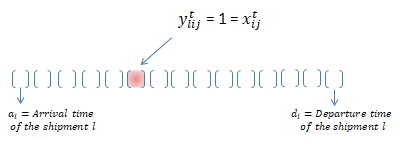
\includegraphics[width=130mm,scale=1.5]{Marco.PNG}
	\caption{Journey of Shipment}
	\label{fig:Journey of Shipment}
\end{figure}

\subsection{Build Up Process}
\label{sec:ParamBUZone}

We define parameters for flights and Build up zones :

\begin{equation*} ${\color{black} Flight k}$ {}  \in {}  ${\color{black}K}$ {} = {} ${\color{black}\{1,2,3,...,K\}}$  \end{equation*} 
\begin{equation*} ${\color{black} BU zone for flight k has Workstations m}$ {}  \in {}  M_k {} = {} ${\color{black}\{1,2..,M\}}$  \end{equation*}
\begin{equation*} ${\color{black} Capacity of ULD in Kgs (W)}$  = 400 \end{equation*}
\begin{equation*} ${\color{black} Weight of each shipment}$  = w_l \end{equation*}
\begin{equation*} ${\color{black} Time taken to build up a ULD in BU zone for Flight k}$  = b_k \end{equation*}
\begin{equation*} ${\color{black} Pre-processing time for each Flight k}$  = p_k \end{equation*}

\subsubsection{Decision Variables for Build Up Process}
\label{sec:DVBDZone}

In the Build Up zone model, the decision needs to be taken regarding which shipments should be assigned to which workstation at what time in a given Build Up zone. For this reason, we introduce a decision variable:  ${z_{lm}^{t}}$

$\newline$
Shipment  \textcolor{black}{$l$} having departure flight  \textcolor{black}{$k$} is assigned to one of  \textcolor{black}{$"m"$} workstations in its BU Zone.
$\newline$

$\textcolor{black}{z_{lm}^{t}\in\{0,1\}, \forall {i \in I, l \in L_i, m \in M_k, t \in T}}$
$\newline$

The second decision we need to take is regarding the number of workstations that need to be allocated to a flight to start its ULD build up process. For this purpose we introduce the second decision variable in BU zone as follows: 

$\newline$
${Q_{mk}^{t}}$ is our binary decision variable to decide if the the Workstation m is assigned to build ULD for Flight k at time t or not. 
$\newline$

$\textcolor{black}{Q_{mk}^{t}\in\{0,1\}, \forall {k \in K, m \in M_k, t \in T}}$
$\newline$
\subsubsection{Constraints for Build Up Process}
\label{sec:constraintsBUZone}

All shipments must be assigned to a workstation in its designated Build up zone.
$\newline$
\begin{align}
\sum_{m \in M}\sum_{t=a_{l}}^{d_l} z_{lm}^{t} = 1  \qquad \forall k \in K, \forall l \in L_k  
\end{align}

$\newline$
If shipments in subset  $\textcolor{black}{l\in\ L_k }$ start at $\textcolor{black}{t}$ in $\textcolor{black}{m^{th}}$  workstation, other shipments in subset $\textcolor{black}{p\in\ L_k \setminus \{ l\} }$ cannot start before $\textcolor{black}{t}$ + $\textcolor{black}{b_{k}}$
$\newline$

\begin{align}
Q_{mk}^{t}\cdot W - \sum_{l\in L_k}z_{lm}^{t}\cdot w_l \ge  \sum_{p\in L_k\setminus \{ l\}}            \sum_{\tau=t+1}^{t+b_k-1} z_{pm}^{\tau}\cdot w_l , \qquad \forall k \in K, \forall m \in M_k, \forall t \in T  
\end{align}

The above simplified form of equation ensures that at any given time t in the set T, which contains time values discretized according to handling time intervals, the capacity of BU zone is never violated.

$\newline$

The number of workstation in the Build up zone that are to be assigned to build ULDs for flight k shall not exceed the number of ULDs that go into the flight and hence we need the following constraint to take care of this.
$\newline$

\begin{align}
\sum_{m \in M_k}\sum_{t=a_l}^{d_k}{Q_{mk}^{t}} \le \dfrac{\sum_{l \in L_k}\sum_{m \in M}\sum_{t=a_l}^{d_k}{z_{lm}^{t} w_{l}}}{W} + 1 ,  \qquad \forall k \in K
\end{align}

$\newline$
If a workstation 'm' in a buildup zone is assigned to flight k at time t, then no other flight can start building its ULDs in that workstation before time t+bk.

$\newline$
\begin{align}
1 - {Q_{mk}^{t}} \ge \sum_{q \in K \setminus \{k\}}  \sum_{\tau = t}^{t + b_{k}}{Q_{mq}^{t}} ,  \qquad \forall k \in K , \forall m \in M_{k}, \forall t \in T
\end{align}

The above equation can also be simplified as follows, when we consider a coarse time discretization as discussed earlier. 
\begin{align}
1 - {Q_{mk}^{t}} \ge Q_{mq}^{t} ,  \qquad \forall k \in K , \forall q \in K \setminus \{k\}, \forall m \in M_{k}, \forall t \in T
\end{align}

%\subsubsection{Precedence constraints}
%\label{sec:ParamBUZone}

In the entire timeline of a shipment from its arrival to departure as in Figure 4, we have a precedence contraint on processes a shipment goes through. The Break down process preceeds the Build up process and hence The assigment for BD zone should happen before Workstation assignment in a BU Zone.

\begin{figure}[hbt!]
	\centering
	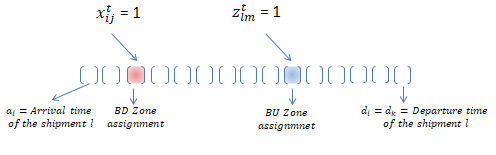
\includegraphics[width=130mm,scale=1.5]{Marco_2.PNG}
	\caption{Journey of Shipment - 2}
	\label{fig:Journey of Shipment - 2}
\end{figure}

The end time of ULD i in Break down process and the summation of transportation time needed to reach Warehouse shall be less that the time at which the shipment l is assigned to a workstation 'm' in Build up zone of flight k.
\begin{align}
 \sum_{j \in J}\sum_{t=a_{l}}^{d_{i}}{\color{black}{(t + h_{j} + T_{j})}} \cdot x_{ij}^t  \le \sum_{m \in M_{k}}\sum_{t=a_{l}}^{d_{l}}z_{lm_{k}}^t \cdot t \qquad \forall i \in I , \forall l \in L_{i}
\end{align}

For Multiple DZ ULDs we have to consider only NRML BD zone assignments for writing precedence constraint : 

\begin{align}
 \sum_{j \in J_{NRML}}\sum_{t=a_{l}}^{d_{i}}{\color{black}{(t + h_{j} + T_{j})}} \cdot x_{ij}^t  \le \sum_{m \in M_{k}}\sum_{t=a_{l}}^{d_{l}}z_{lm_{k}}^t \cdot t \qquad \forall i \in I , \forall l \in L_{i}
\end{align}

Slack for each shipment is given by difference in departure time and the time at which shipments are built up into ULDs. Let this slack time for each shipment be greater than ${s_{min}}$

\begin{align}
 ( d_{l} + p_{k}) - (\sum_{t=a_{l}}^{d_{l}}z_{lm_{k}}^t \cdot (t + b_{k}) )  \ge s_{min} \qquad \forall i \in I, \forall l \in L_{i}, \forall k \in K, \forall t \in T
\end{align}
\begin{align}
s_{min} \ge 0
\end{align}

\subsection{Objective Function}
\label{sec:objBUZone}

By maximizing the minimum slack of all shipments, we ensure that each shipment is ready well before its departure time.

\begin{equation*}
\max s_{min}
\end{equation*}


\subsection{Alternate Model for Build Up Process}
\label{sec:ParamBUZone}

In this alternate model, we define the following for the flights and the time horizons. 

\begin{equation*} ${\color{black} Flight k}$ {}  \in {}  ${\color{black}K}$ {} = {} ${\color{black}\{1,2,3,...,K\}}$  \end{equation*} 
\begin{equation*} ${\color{black} Time horizon t}$ {}  \in {}  ${\color{black}T}$ {} = {} ${\color{black}\{1,2,3,...,T\}}$ \end{equation*} 

$\newline$

The first constraint is about available weight of shipment of flight k at any time t , which means the summation of the weights of the seperate shipments which are waiting in the warehouse and ready to be built up.

$\newline$

$avail_{kt}$ $\in$ $\mathbb{R}$

$\newline$

The second one is the due time of the build up process for a flight k.

$\newline$

$due_{k}$ $\in$ $\mathbb{R}$

$\newline$

The third one is the total shipment weight as a demand for a flight k.

$\newline$

$dem_{k}$ $\in$ $T$

$\newline$

The fourth one is the maximum number of ULDs building up simultaneously for a flight k. It actually means number of workstations which are working parallel. In practice we only want to build a limited number of ULDs for the same flight at the same time. This leaves more options and time to react to operational problems during build up and allows to build the ULDs on close-by workstations. Let maximum split denote the maximum desired number of parallel build-ups of a flight. Enforcing a hard limit in practice might lead to offloads for flights where the shipment arrives rather late such that the limit is too low to build all ULDs on time. In these cases we want to set a less restrictive limit.


As a suitable limit we choose the maximum required parallel build-ups, between any build-up period and the scheduled departure period of the flight, for which all shipments can be packed. For each period t, we determine the shipment weight arriving in the future (weight demand of flight k) $-$ (available weight at time t for flight k) and the weight that could be packed in the remaining time, if no parallel build-ups are allowed. Note that the number of ULDs that can be built sequentially in the time between t and due time for flight k, can be determined as (due date of flight k $-$ t $-$ 1) $/$ (duration to build a ULD for a flight k). The ratio of both gives us the required parallelism and its maximum over the periods the sought limit. If the required parallelism is less than the desired maximum split, we allow maximum split to be built in parallel.

$\newline$

$split_{k}$ $\in$ $\mathbb{N}$

$\newline$

The fifth parameter is the number of ULDs scheduled for a flight k. It means that total shipment weight for a flight k is divided into capacity which is 400 kg and gives us the value of the parameter. 

$\newline$

$uld_{k}$ $\in$ $\mathbb{N}$

$\newline$

The sixth one is the duration in minutes for building a ULD for flight k. We actually know which BU zone is used for flight k before, that is why we do not consider here BU zone index.

$\newline$

$dur_{k}$ $\in$ $\mathbb{N}$

$\newline$

The seventh one is the weight of an ULD which is 400 kg as stated in the data.

$\newline$

$cap$ $\in$ $\mathbb{R}$

$\newline$

The last one is the number of workstations handling the ULDs during time t. It is for all flights in time horizon t.
$\newline$
$open_{t}$ $\in$ $\mathbb{N}$

$\newline$


\subsubsection{Decision Variables for Build Up Process}
\label{sec:DVBUZone}

The primary decision made by the model is the number of ULDs to start building at each period. To calculate the objective value, we introduce further decision variables. One part of the objective is to load as much as possible. There are two reasons that might prevent us from achieving this goal: First, if not all ULDs can be scheduled for build-up. Second, if a ULD is scheduled before enough shipment is available. We capture the effect of each reason in one variable.

$\newline$

$\textcolor{black}{start_{kt}\in\mathbb{N}, \forall {k \in K, t \in T}}$ : Number of ULDs started to build at time t for a flight k $t \le due_{k} $ - $dur_{k}$

$\newline$

$\textcolor{black}{offload_{k}\in\mathbb{N}, \forall {k \in K}}$ : Number of NOT scheduled ULDs for flight k


$\newline$

$\textcolor{black}{dead_{kt}\in\mathbb{R} \ge 0, \forall {k \in K, t \in T}}$ : Lost weight of shipments on flight k if ULDs are built before enough shipments available at time t


$\newline$

\subsubsection{Constraints for Build Up Process}
\label{sec:constraintsBUZone}

There is no technical reason to restrict the number of ULDs that are built in parallel for a segment. However, in practice there might occur problems during
a build-up when an item cannot be packed onto the planned ULD. In this case, the load planner has to find another ULD with enough remaining capacity under massive time pressure. The more ULDs that are not started yet, the more options and time he has for replanning. Furthermore, if only a few ULDs for a segment are built in parallel, they can be assigned to spatially close workstations. This might reduce transport distances and improve overview during build-up. We note that, during a period t, the ULDs that were started during period (t $-$ $dur_{k}$ $+$ 1) to period t are still work in progress. For each flight k we limit the number of simultaneously built ULDs by splitk as:

\begin{align}
\sum_{t' \in {T}} start_{kt'} \le split_{k} \qquad \forall k \in K, \forall t \in T
\end{align} $t - dur_{k} \le t' \le t$

$\newline$

The number of usable workstations is limited. As each workstation can process one ULD at a time, we limit the number of simultaneously processed ULDs during period t by $open_{t}$. To calculate this number for a point in time, we sum up the ULDs of all flights that have been started during earlier periods and are not finished yet:

\begin{align}
\sum_{k \in {K}}\sum_{t' \in {T}} start_{kt'} \le open_{t} \qquad \forall t \in T
\end{align} $t - dur_{k} \le t' \le t$

$\newline$

\subsection{Objective Function for Alternate model}
\label{sec:objBUZone}

While satisfying all the given constraints, we want to load as much cargo as possible. o maximize the load, we minimize the amount of weight the departing flight lost and the number of ULDs building up unassociated to the departing flight.

\begin{equation*}
\min \qquad {} (\sum_{k \in K} \sum_{t \in T} dead_{kt} + \sum_{k \in K} offload_{k})
\end{equation*}

$\newline$


\section{Solution and Discussion}
\label{sec:modeloutput}

We implemented all above presented variables and constraints in python using Jupyter notebook. We checked the notebook in both Linux and Windows 64-bit operating systems and it compile without any errors in both. As a MIP solver we used Gurobi in version 8.1.0. For data cleaning Pandas(0.24.0) and Numpy(1.15.4) was used. All the graphs generated using matplotlib(3.0.2).

$\newline$
We perform our testing in two machines. One machine had Intel Core i7-4500U processor with 2 cores clocked at 1.8 GHz and equipped with 4 MB cache running on a 64-bit Ubuntu 18.04 lts. Another machine had Intel Core i7-6500U  processor with 2 cores clocked at 2.5 GHz and equipped with 4 MB cache running on a 64-bit Windows 10.  Each machine had 8 GB main memory and all the experiments were performed under full load.

$\newline$
First model takes three hours to build the entire model and for the second model takes around two hours to build entire model, probably due to a very fine time discretization that we used (We can improve the time by using a coarse discretization of time). In the solution, we see that all shipments catch their flights on time as was our goal in this project. To choose a planning time horizon that fits our needs, we evaluated different planning time horizons with repect to the solution quality and the runtime. For the BD zones, first we determined the planning horizon as one minute but it took a lot of time for the solution. Then we decided to discretize the time using handling time intervals for each BD zone. For the BU zones, time is discretized in one minute intervals.

\subsection{Break down zone results}
\label{sec:fmBDResults}
The results for the BD zones are visualized in both Figure 5 and Figure 6. Most number of ULDs allocated to BD NRML-1 because transportation time and the handling time for this particular BD zone are less than the others. Similarly this is applied to the ULD which is containing animals. For this ULDs BD NML-3 was selected most. Hence, our model picked the best BD zone. As per the data we received it used only three normal break down zones and three animal break down zones. Other break down zones are not picked by our model for this data. 


\begin{figure}[hbt!]
	\centering
	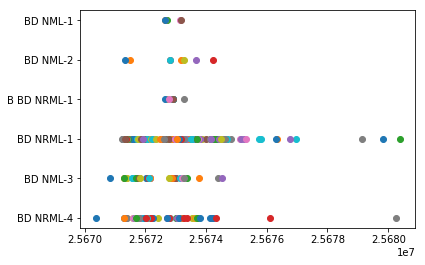
\includegraphics[width=150mm,scale=1.0]{bd_assignment.png}
	\caption{Shipment Arrival Times (X-axis) and BD Zones (Y-axis)}
	\label{fig:Shipment Arrival Times (X-axis) and BD Zones (Y-axis)}
\end{figure}

\begin{figure}[hbt!]
	\centering
	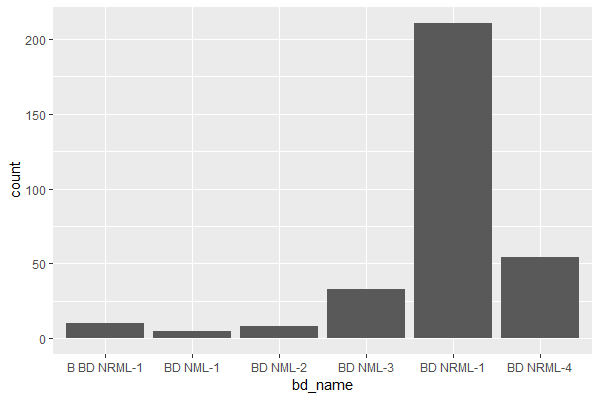
\includegraphics[width=150mm,scale=1.0]{Rplot_bd.png}
	\caption{BD zones (X-axis) and ULD count (Y-axis)}
	\label{fig:BD zones (X-axis) and ULD count (Y-axis)}
\end{figure}

$\newline$
$\newline$
\subsection{Build-up zone results - main model}
\label{sec:fmBDResults}
The results for the BD zones are visualized in both Figure 5 and Figure 6. Most number of ULDs allocated to BD NRML-1 because transportation time and the handling time for this particular BD zone are less than the others. Similarly this is applied to the ULD which is containing animals. For this ULDs BD NML-3 was selected most. Hence, our model picked the best BD zone. As per the data we received it used only three normal break down zones and three animal break down zones. Other break down zones are not picked by our model for this data.

\begin{figure}[hbt!]
	\centering
	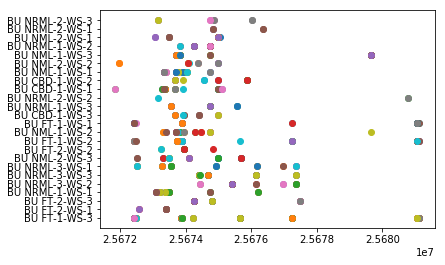
\includegraphics[width=150mm,scale=1.0]{bu_assignment.png}
	\caption{Shipment Arrival Times (X-axis) and BD Zones (Y-axis)}
	\label{fig:Shipment Arrival Times (X-axis) and BD Zones (Y-axis)}
\end{figure}

\begin{figure}[hbt!]
	\centering
	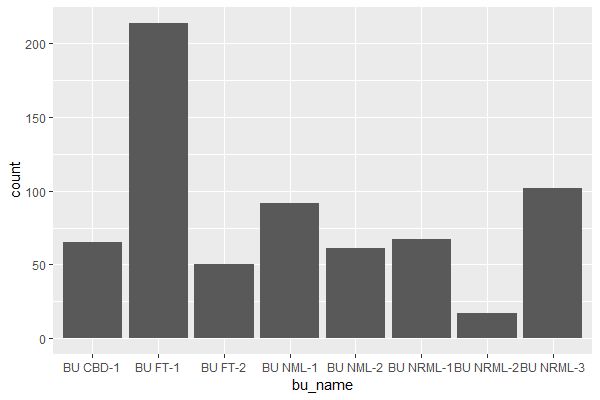
\includegraphics[width=150mm,scale=1.0]{Rplot_bu.png}
	\caption{BD zones (X-axis) and ULD count (Y-axis)}
	\label{fig:BD zones (X-axis) and ULD count (Y-axis)}
\end{figure}

\pagebreak
\subsection{Build-up zone results - alternative model}
\label{sec:fmBDResults}
The results for the BD zones are visualized in both Figure 5 and Figure 6. Most number of ULDs allocated to BD NRML-1 because transportation time and the handling time for this particular BD zone are less than the others. Similarly this is applied to the ULD which is containing animals. For this ULDs BD NML-3 was selected most. Hence, our model picked the best BD zone. As per the data we received it used only three normal break down zones and three animal break down zones. Other break down zones are not picked by our model for this data.

\begin{figure}[hbt!]
	\centering
	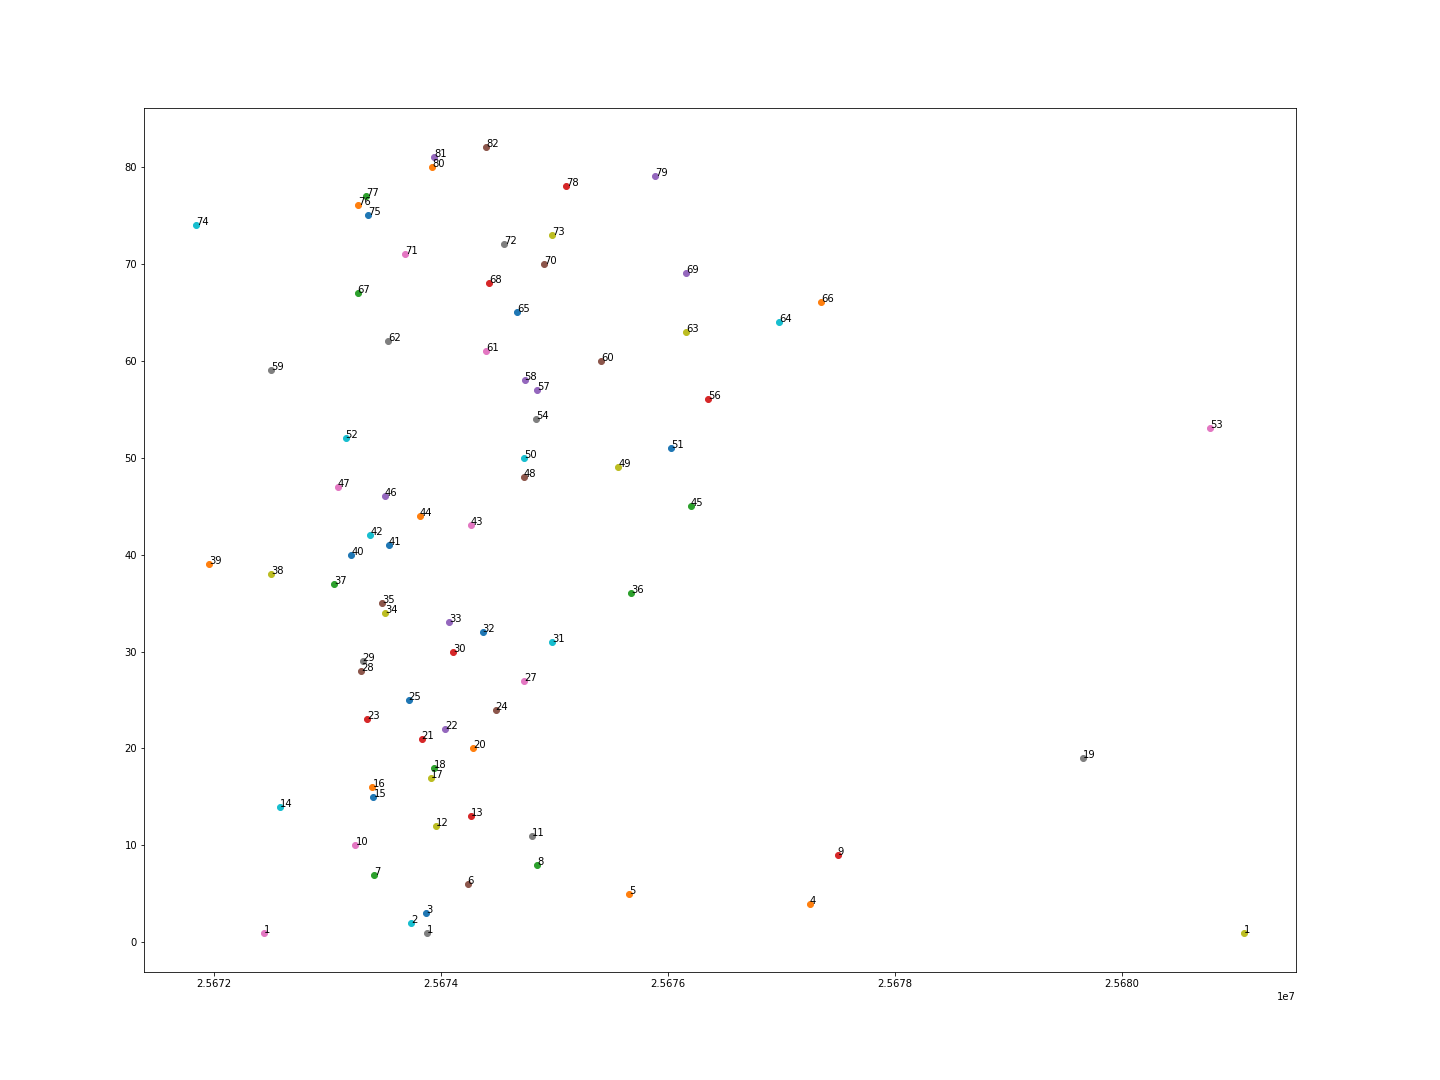
\includegraphics[width=150mm,scale=1.0]{al_model_2.png}
	\caption{Shipment Arrival Times (X-axis) and BD Zones (Y-axis)}
	\label{fig:Shipment Arrival Times (X-axis) and BD Zones (Y-axis)}
\end{figure}

%\subsection{Overall Model}
%\label{sec:overallModel}

%------------------------------------------------------------------------

%\begin{table}[h!]
%	\begin{center}
%		\caption{Drop Zone}
%		\label{tab:table1}
%		\begin{tabular}{l|c|c} % <-- Alignments: 1st column left, 2nd middle and 3rd right, with vertical lines in between
%			\textbf{Name} & \textbf{Workstations} & \textbf{Sequence}\\
%			\hline
%			& & \\
%			DZ NRML-1 & 6 & 1\\
%			DZ NRML-2 & 4 & 2\\
%			DZ NML-1 & 3 & 3\\
%			DZ CLD-1 & 5 & 4\\
%		\end{tabular}
%	\end{center}
%\end{table}

%\begin{table}[h!]
%	\begin{center}
%		\caption{Break Down Zone}
%		\label{tab:table1}
%		\begin{tabular}{l|c|c|c|c} % <-- Alignments: 1st column left, 2nd middle and 3rd right, with vertical lines in between
%			\textbf{Name} & \textbf{Workstations} & \textbf{Sequence} & \textbf{ToWH} & \textbf{HandTimePerULD}\\
%			\hline
%			& & & & \\
%			B BD NRML-1 & 33 & 1 & 0:30 & 0:24\\
%			B BD NRML-2 & 10 & 2 &  0:25 & 0:24\\
%			BD NML-1 & 4 & 3 &  0:40 & 0:13\\
%			BD CLD-1 & 8 & 4  &  0:30 & 0:17\\
%			BD NRML-1 & 5 & 5  &  0:30 & 0:20\\
%			BD NML-2 & 3 & 6  & 0:25 & 0:13\\
%			BD NRML-2 & 6 & 7  & 0:40 & 0:20\\
%			BD NRML-3 & 3 & 8  & 0:40 & 0:20\\
%			BD CLD-2 & 5 & 9  & 0:30 & 0:17\\
%			BD NML-3 & 5 & 10  & 0:25 & 0:20\\
%			BD NRML-4 & 3 & 11  & 0:30 & 0:13\\
%			BD CLD-4 & 1 & 12  & 0:40 & 0:15\\
%		\end{tabular}
%	\end{center}
%\end{table}

\end{document}